%----------------------------------------------------------------------------
\section{Monitor forráskód generátor}
%----------------------------------------------------------------------------

%----------------------------------------------------------------------------
\subsection{A monitor interfészei}
%----------------------------------------------------------------------------

\begin{figure}[h!]
    \centering
    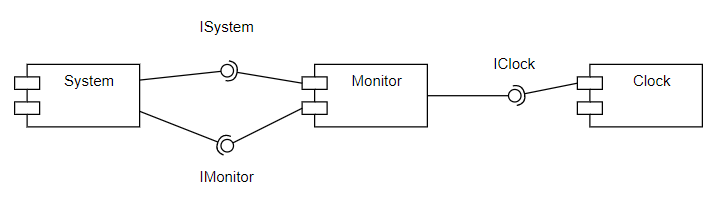
\includegraphics[width=130mm, keepaspectratio]{figures/monitor_architecture.png}
    \caption{Monitor architektúra diagram.}
	\label{monitor_architecture}
\end{figure}

A \ref{monitor_architecture} ábrán látható a megfigyelt rendszer és a monitorhoz tartozó architektúra diagram.
A monitorozás alatt lévő rendszer egy \textit{IMonitor} interfészen keresztül kommunikál a monitorral.
Az interfész \textit{Java} implementációja a \ref{IMonitor_interface} kódrészleten tekinthető meg.
A monitor azt vizsgálja, hogy a rendszer a szcenárió szerint viselkedik-e.
Monitornak a következő interfészt kell megvalósítania:
\begin{itemize}
    \item \textit{update()}: ezzel a függvénnyel lehet továbbítani a rendszer üzeneteit a monitor számára.
	Bemenetként az üzenet feladóját, címzettjét, nevét és paramétereit kapja.
	A monitor frissíti a belső automatájának állapotát.
    \item \textit{goodStateReached()}: a rendszer ezen a függvényen keresztül kérdezi le a monitortól, hogy jó állapotban van-e a követelmény szempontjából, azaz nem történt e hiba.
    Visszatérési értéke egy \textit{boolean} érték.
    \item \textit{requirementSatisfied()}: a rendszer ezzel a függvénnyel kérdezheti le, megfelel-e a követelménynek.
    Visszatérési értéke egy \textit{boolean} érték.
	\item \textit{errorDetected()}: ez a függvény tartalmazza a hibaelhárító funkcionalitás implementációját.
	A rendszer ezt a függvényt használhatja erre a célra hiba esetén.
	Bemenetként azt az üzenetet kapja meg, amely hatására előjött a hiba az \textit{update()} függvényhez hasonlóan.
    \item \textit{noMoreMessages()}: a rendszer ezen a függvényen keresztül jelzi a monitornak a kommunikáció végét.
\end{itemize}

Az üzenetek megfigyeléséhez szükséges segédfüggvényeket a kommunikációs infrastruktúrához kézzel kell megírni.
Ezek a monitort az \textit{update()} függvényen keresztül hívják.

\begin{lstlisting}[language=java,frame=single, float=h!, caption={Monitor interfész Java implementációja.},captionpos=b,label=IMonitor_interface]
public interface IMonitor {
	public boolean goodStateReached();
	public void update(String sender, String receiver, String messageType, Map<String, Object> parameters);
	public boolean requirementSatisfied();
	public void errorDetected(String sender, String receiver, String messageType, Map<String, Object> parameters);
	public void noMoreMessages();
}
\end{lstlisting}

Az időzítési feltételek kiértékelése érdekében a monitornak szüksége van egy időzítő komponensre.
Az időzítő komponenshez tartozik egy időzítő interfész amin keresztül elérhető a komponens.
Ezen az interfészen keresztül lehet az óraváltozókat lekérdezni vagy nullázni.
Két függvénye van:

\begin{itemize}
    \item \textit{getClock(String clock)}: óraváltozó lekérdezése név alapján.
    \item \textit{resetClock(String clock)}: óraváltozó nullázása név alapján.
\end{itemize}

\begin{lstlisting}[language=java,frame=single, float=h!, caption={Időzitő interfész Java implementációja.},captionpos=b,label=IClock_interface]
public interface IClock {
	public long getClock(String clock);
	public void resetClock(String clock);
}
\end{lstlisting}

A \ref{IClock_interface} kódrészlet tartalmazza az időzítő interfész implementációját, a \textit{IClock} \textit{Java} interfészt.

A monitor az \textit{ISystem} interfészen keresztül tud a rendszernek üzeneteket küldeni a megfigyelt viselkedésről.
Ezt az interfészt a monitorozott rendszer valósítja meg.
Három függvénye van:
\begin{itemize}
	\item \textit{receiveMonitorStatus()}: a monitor jelzi a rendszer felé a követelmény alapján az aktuális státuszt.
	Bementként a monitor által küldött üzenetet kapja meg.
	\item \textit{receiveMonitorError()}: a monitor jelzi a rendszer felé ha hibát detektált.
	Bemenetként két üzenetet kap: a hibát okozó üzenetet és az utolsó üzenetet, amikor még a rendszer jó állapotban volt a követelmény szempontjából.
	\item \textit{receiveMonitorSuccess()}: a monitor jelzi a rendszer felé ha teljesült a követelmény.
\end{itemize}

\begin{lstlisting}[language=java,frame=single, float=h!, caption={Rendszer interfész Java implementációja.},captionpos=b, label=ISystem_interface]
public interface ISystem {
	public void receiveMonitorStatus(String message);
	public void receiveMonitorError(String actualMessage, String lastAcceptedMessage);
	public void receiveMonitorSuccess();
}
\end{lstlisting}

Az \ref{ISystem_interface}-es kódrészlet tartalmazza az \textit{ISystem} java interfészt.

%----------------------------------------------------------------------------
\subsection{A monitor forráskód megvalósítása}
%----------------------------------------------------------------------------
A generált forráskód struktúrája egy statikus és egy generált dinamikus részből áll.
A statikus részbe az időzített automata \textit{Java} osztályai kerülnek:
\begin{itemize}
    \item State: egy állapotot leíró osztály
    \item Transition: egy átmenetet reprezentáló osztály
    \item Automaton: egy automatát megvalósító osztály
\end{itemize}
Ezek segédosztályok, amelyek a generált automata reprezentálására szolgálnak.
A statikus rész a \textit{hu.bme.mit.dipterv.text.util} csomagban található meg, amely a \ref{util_csomag} ábrán látható.

A monitor interfész, a monitor Java osztálya, az időzítő interfész és a hozzá tartozó java osztály is ebbe a részbe tartozik.

A dinamikus részben található a \textit{Specification} Java osztály, ami a szcenárió alapján generált automata forráskódját tartalmazza.
Az osztály konstruktorába jön létre egy \textit{Automaton} objektum, amihez hozzáadjuk a leírás alapján a megfelelő állapotokat és átmeneteket \textit{State} és \textit{Transition} objektumokat használva.

\begin{figure}[!ht]
    \centering
    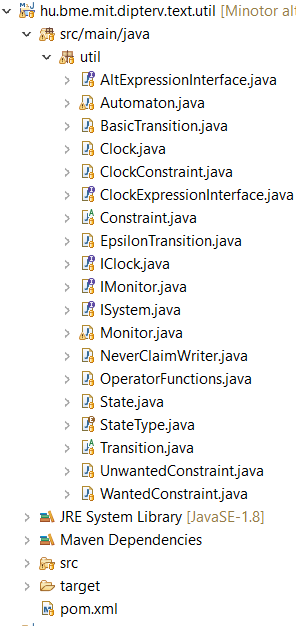
\includegraphics[width=180mm, height= 13cm, keepaspectratio]{figures/util_csomag.png}
    \caption{Az \textit{util} csomag tartalma.}
	\label{util_csomag}
\end{figure}

A szükséges forráskódok generálásához az \textit{Xtend} technológiát használtam.

%----------------------------------------------------------------------------
\clearpage\subsection{Mintapélda}
%----------------------------------------------------------------------------

A \ref{mintapélda} kódrészleten látható egy szcenárió követelmény szöveges leírása, amit egy okos telefon működésére specifikáltunk.
A \ref{monitor_visualisation} ábrán látható a leíráshoz tartozó diagram vizualizációja, az \ref{okos_nc} kódrészlet pedig a generált automata leírását tartalmazza.

Az okos telefonon van egy zene lejátszási lista generáló alkalmazás.
A követelményben azt várjuk el, hogy ha a felhasználó megnyitja az alkalmazást akkor a belső kamera készít az arcáról egy képet.
A kép alapján eldönti, hogy milyen a felhasználó kedve és az alapján előállít egy zene lejátszási listát.

A \ref{okos_kapcsolat} kódrészleten látható az okos telefon és a monitor közti kapcsolat megvalósítása \textit{Java} kódban.
A rendszerben lévő \textit{User}, \textit{Device} és \textit{Database} osztályok mind attribútumként átveszik a \textit{Monitor} osztályt, amely megvalósítja az \textit{IMonitor} interfészt.

\begin{lstlisting}[frame=single, float=ht!, caption={Okos telefon működésére megadott szcenárió követelmény.},captionpos=b, label=mintapélda]
specification Photo{

	object User user;
	object Device device;
	object Database db;

	constraint error {
		message closeApp() user -> device;
	}

	scenario playlist_generation{
		message openApp() user -> device;
		message accessWebcam() device -> device;
		required message getPhoto() device -> user;
		fail message cameraOffline() user -> device;
		required strict message retrieveMood() device -> db;
		required message retrieveMusic() device -> db;
		strict message generatePlaylist() db -> device;
	}
}
\end{lstlisting}

\begin{figure}[!ht]
    \centering
    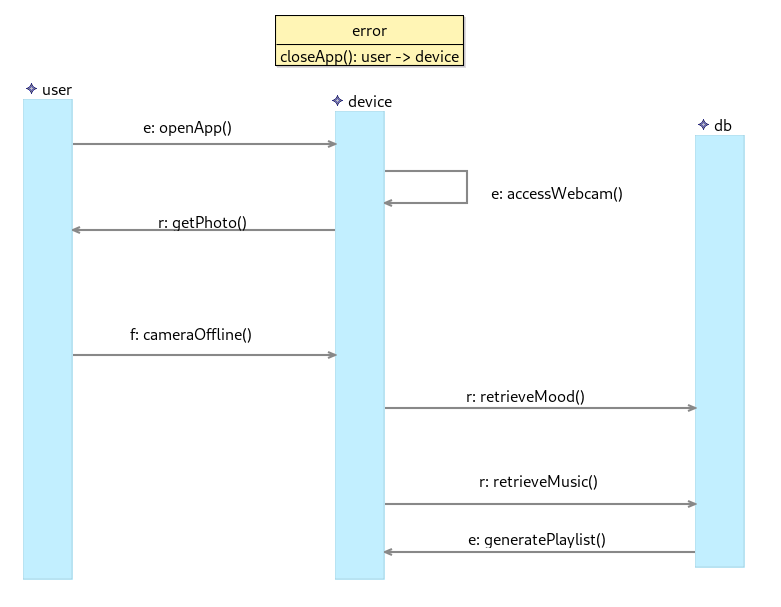
\includegraphics[width=150mm, keepaspectratio]{figures/monitor_device_visualisation_diagram.png}
    \caption{A \ref{mintapélda} leíráshoz tartozó diagram.}
	\label{monitor_visualisation}
\end{figure}

\begin{lstlisting}[frame=single, float=ht!, caption={Generált automata Never claim formátumba.},captionpos=b,label=okos_nc]
never{ /*playlist_generationMonitor*/
T0_init:
 if
 :: (!(user.openApp().device)) -> goto T0_init
 :: (user.openApp().device) -> goto T0_q1
 fi;
T0_q1:
 if
 :: (!(device.accessWebcam().device)) -> goto T0_q1
 :: (device.accessWebcam().device) -> goto T0_q2
 fi;
T0_q2:
 if
 :: (!(device.getPhoto().user)) -> goto T0_q2
 :: (!(device.getPhoto().user)) -> goto accept_q3
 :: (device.getPhoto().user) -> goto T0_q4
 fi;
accept_q3:
 if
 fi;
T0_q4:
 if
 :: (!(user.cameraOffline().device)) -> goto T0_q6
 :: (!(user.cameraOffline().device)) -> goto T0_q4
 :: (user.cameraOffline().device) -> goto accept_q5
 fi;
accept_q5:
 if
 fi;
T0_q6:
 if
 :: (device.retrieveMood().db) -> goto T0_q8
 :: (!(device.retrieveMood().db)) -> goto accept_q7
 fi;
accept_q7:
 if
 fi;
T0_q8:
 if
 :: (!(device.retrieveMusic().db)) -> goto T0_q8
 :: (!(device.retrieveMusic().db)) -> goto accept_q9
 :: (device.retrieveMusic().db) -> goto T0_q10
 fi;
accept_q9:
 if
 fi;
T0_q10:
 if
 :: (db.generatePlaylist().device) -> goto T0_q11
 fi;
T0_q11:
 if
 fi;
}
\end{lstlisting}

\begin{lstlisting}[language=java, frame=single, float=ht!, caption={Az okos telefon és hozzá tartozó monitor fel konfigurálásának Java implementációja.},captionpos=b,label=okos_kapcsolat]
public class Main {
	public static void monitorStatus(String status) {
		System.out.println(status);
	}

	public static void main(String[] args) {
		Specification specification = new Specification();
		specification.listAutomatas();
		IMonitor monitor = new Monitor(specification.getAutomata().get(0));

		User user = new User();
		Device device = new Device();
		Database db = new Database();
		user.device = device;
		device.user = user;
		device.db = db;
		db.device = device;
		user.monitor = monitor;
		device.monitor = monitor;
		db.monitor = monitor;

		user.init();
	}
}
\end{lstlisting}

\begin{lstlisting}[language=java, frame=single, float=ht!, caption={Az okos telefon Java osztálya.},captionpos=b,label=okos_device]
public class Device {
	public IMonitor monitor;
	public User user;
	public Database db;

	void openApp() {
		monitor.update("user", "device", "openApp", new HashMap<String, Object>());
		accessWebcam();
	}

	void accessWebcam() {
		monitor.update("device", "device", "accessWebcam", new HashMap<String, Object>());
		user.getPhoto();
		db.retrieveMood();
		db.retrieveMusic();
	}

	void cameraOffline() {
		monitor.update("user", "device", "cameOffline", new HashMap<String, Object>());
	}

	void generatePlaylist() {
		monitor.update("db", "device", "generatePlaylist", new HashMap<String, Object>());
	}
}
\end{lstlisting}

A \ref{okos_device} kódrészlet az okos telefon \textit{Java} osztálya.
Megtekinthető a monitor és az eszköz közti kommunikáció megvalósítása is.
A \textit{Device} osztály a tágváltozójaként tárolt \textit{IMonitor}-nak küldi az üzeneteket az \textit{update()} függvény használatával.

\begin{lstlisting}[language=java, frame=single, float=ht!, caption={Monitor kimenete a rendszer működésének egyes fázisaiban.},captionpos=b,label=okos_monitor]
Received Message: user.openApp().device
q1
[System] Received status from monitor: System is in good state.
[Clock] reset x
Received Message: device.accessWebcam().device
q2
[System] Received status from monitor: System is in good state.
Received Message: device.getPhoto().user
q5
[System] Received status from monitor: System is in good state.
Received Message: someone.message().else
q7
[System] Received status from monitor: System is in good state.
Received Message: device.retrieveMood().db
q9
[System] Received status from monitor: System is in good state.
Received Message: device.retrieveMusic().db
q11
[System] Received status from monitor: System is in good state.
Received Message: db.generatePlaylist().device
q12
[System] Received status from monitor: System is in good state.
[System] Received status from monitor: Requirement satisfied
\end{lstlisting}

A \ref{okos_monitor} kódrészleten látszik, hogy a rendszer a működése elején nem felelt meg a monitor követelményének.
Amikor a működése végére ért akkor a monitor jelezte, hogy a rendszer jó állapotban van a „\textit{Good state}” üzenettel és, hogy a követelmény teljesült a "\textit{Requirement Satisfied}" üzenettel.
A mintapéldához tartozó \textit{Specification} osztály a \textit{Függelékben} található (\ref{specification_class}).
A generált automatát a konstruktorában állítja elő.

%----------------------------------------------------------------------------
\clearpage\subsection{Összetett szerkezetek}
%----------------------------------------------------------------------------

A monitor forráskód generátor támogatja az \textit{alt}, \textit{par} vagy \textit{loop} operátorokat tartalmazó szcenáriókat is.
Ezt funkcionalitást a tesztelés során mutatom be részletesebben.

%----------------------------------------------------------------------------
\subsection{Időzítési feltételek}
%----------------------------------------------------------------------------

A monitor forráskód generátor támogatja az időzítési feltételeket tartalmazó szcenáriókat is.
A \ref{computer_scenario} kódrészletben található szcenárió első üzenetén a "\textit{reset x}" címke jelzi a monitornak, hogy az "\textit{x}" óraváltozót nullázni kell.
Egy óraváltozó felvételét is a "\textit{reset}" címkével lehet végrehajtani.
Ezt az óraváltozót használhatjuk majd a szcenáriónk későbbi üzeneteinél időzítési feltételek megadására.
Például a \ref{computer_scenario} kódrészletben lévő szcenárió esetén, ha a monitor megkapja a \textit{checkEmail()} üzenetet, akkor létrehozz egy "\textit{x}" óraváltozót mivel ilyen még nem létezett előtte.
Ha a szcenárió végére érünk és a monitor megkapja a \textit{downloadEmail()} üzenetet, akkor a monitor kiértékeli az üzeneten lévő időzítési feltételt az óraváltozóban tárolt időérték alapján.
Ha az előbbi feltétel teljesült akkor tovább lépteti az időzített automatát.
A \ref{computer_main} kódrészlet a példához tartozó \textit{Main} \textit{Java} osztály leírását tartalmazza, a \ref{computer_java} kódrészlet pedig a rendszerhez tartozó \textit{Computer} \textit{Java} osztályt.
A \ref{computer_monitor} kódrészleten megtekinthető a monitor kimenete.
A kimenet végén lévő "\textit{System is in good state.}" üzenet jelzi, hogy a rendszer jó állapotban van.

\begin{lstlisting}[language=java, frame=single, float=ht!, caption={Időzítési feltételeket tartalmazó szcenárió},captionpos=b,label=computer_scenario]
specification Email {

	object Computer computer;
	object Server server;

	clock x;

	constraint constraints{
		message logout() computer -> server;
	}

	constraint c {
		message login() server -> computer;
	}

	scenario sendEmail{
		message checkEmail() computer -> computer reset x;
		message sendUnsentEmail() required computer -> server;
		message newEmail() computer -> server pastConstraint {constraints};
		message downloadEmail() computer -> server clockConstraint {x < 10};
	}
}
\end{lstlisting}

\begin{lstlisting}[language=java, frame=single, float=ht!, caption={Időzítéses példához tartozó Main osztály.},captionpos=b,label=computer_main]
public class Main {
	public static void monitorStatus(String status) {
		System.out.println(status);
	}

	public static void main(String[] args) {
		Specification specification = new Specification();
		specification.listAutomatas();
		IClock clock = new Clock();
		IMonitor monitor = new Monitor(specification.getAutomata().get(0), clock);

		Server server = new Server(monitor);
		Computer computer = new Computer(server, monitor);
	}
}
\end{lstlisting}

\begin{lstlisting}[language=java, frame=single, float=ht!, caption={A Computer java osztálya.},captionpos=b,label=computer_java]
public class Computer {
	public Server server;
	public IMonitor monitor;

	Computer(Server server, IMonitor monitor) {
		this.server = server;
		this.monitor = monitor;
		monitor.update("computer", "computer", "checkEmail", new HashMap<String, Object>());
		checkEmail();
	}

	void checkEmail() {
		monitor.update("computer", "server", "sendUnsentEmail", new HashMap<String, Object>());
		server.sendUnsentEmail();

		monitor.update("computer", "server", "newEmail", new HashMap<String, Object>());
		server.newEmail();

		monitor.update("computer", "server", "downloadEmail", new HashMap<String, Object>());
		server.downloadEmail();
	}
}
\end{lstlisting}

\begin{lstlisting}[language=java, frame=single, float=ht!, caption={Időzítéses példa monitor kimenete.},captionpos=b,label=computer_monitor]
Received Message: computer.checkEmail().computer
q1
[System]Received status from monitor: System is in good state.
Received Message: computer.sendUnsentEmail().server
q3
[System]Received status from monitor: System is in good state.
Received Message: computer.newEmail(receiver, subject).server
q4
[System]Received status from monitor: System is in good state.
Received Message: computer.downloadEmail(timeout).server
q5
[System]Received status from monitor: System is in good state.
[System]Received status from monitor: Requirement satisfied
\end{lstlisting}

Az óraváltozók és időzítések megvalósításához az "\textit{org.apache.commons.lang3}" könyvtár "\textit{time}" csomag \textit{StopWatch} osztályát használtam.
Ha az automata élén van egy időzítési feltétel akkor a monitor komponens az időzítő komponenstől elkéri a feltételben szereplő óraváltozóban tárol időt és kiértekeli a feltételt.
Ha a feltétel teljesül, akkor az időzítés szempontjából a tranzíció megtörténhet.
A monitor akkor jelez hibát ha az átmeneten lévő időzítési feltétel nem teljesült és az üzenet más átmenetre se illeszkedik.